% Options for packages loaded elsewhere
\PassOptionsToPackage{unicode}{hyperref}
\PassOptionsToPackage{hyphens}{url}
%
\documentclass[
]{article}
\usepackage{amsmath,amssymb}
\usepackage{iftex}
\ifPDFTeX
  \usepackage[T1]{fontenc}
  \usepackage[utf8]{inputenc}
  \usepackage{textcomp} % provide euro and other symbols
\else % if luatex or xetex
  \usepackage{unicode-math} % this also loads fontspec
  \defaultfontfeatures{Scale=MatchLowercase}
  \defaultfontfeatures[\rmfamily]{Ligatures=TeX,Scale=1}
\fi
\usepackage{lmodern}
\ifPDFTeX\else
  % xetex/luatex font selection
\fi
% Use upquote if available, for straight quotes in verbatim environments
\IfFileExists{upquote.sty}{\usepackage{upquote}}{}
\IfFileExists{microtype.sty}{% use microtype if available
  \usepackage[]{microtype}
  \UseMicrotypeSet[protrusion]{basicmath} % disable protrusion for tt fonts
}{}
\makeatletter
\@ifundefined{KOMAClassName}{% if non-KOMA class
  \IfFileExists{parskip.sty}{%
    \usepackage{parskip}
  }{% else
    \setlength{\parindent}{0pt}
    \setlength{\parskip}{6pt plus 2pt minus 1pt}}
}{% if KOMA class
  \KOMAoptions{parskip=half}}
\makeatother
\usepackage{xcolor}
\usepackage[margin=1in]{geometry}
\usepackage{color}
\usepackage{fancyvrb}
\newcommand{\VerbBar}{|}
\newcommand{\VERB}{\Verb[commandchars=\\\{\}]}
\DefineVerbatimEnvironment{Highlighting}{Verbatim}{commandchars=\\\{\}}
% Add ',fontsize=\small' for more characters per line
\usepackage{framed}
\definecolor{shadecolor}{RGB}{248,248,248}
\newenvironment{Shaded}{\begin{snugshade}}{\end{snugshade}}
\newcommand{\AlertTok}[1]{\textcolor[rgb]{0.94,0.16,0.16}{#1}}
\newcommand{\AnnotationTok}[1]{\textcolor[rgb]{0.56,0.35,0.01}{\textbf{\textit{#1}}}}
\newcommand{\AttributeTok}[1]{\textcolor[rgb]{0.13,0.29,0.53}{#1}}
\newcommand{\BaseNTok}[1]{\textcolor[rgb]{0.00,0.00,0.81}{#1}}
\newcommand{\BuiltInTok}[1]{#1}
\newcommand{\CharTok}[1]{\textcolor[rgb]{0.31,0.60,0.02}{#1}}
\newcommand{\CommentTok}[1]{\textcolor[rgb]{0.56,0.35,0.01}{\textit{#1}}}
\newcommand{\CommentVarTok}[1]{\textcolor[rgb]{0.56,0.35,0.01}{\textbf{\textit{#1}}}}
\newcommand{\ConstantTok}[1]{\textcolor[rgb]{0.56,0.35,0.01}{#1}}
\newcommand{\ControlFlowTok}[1]{\textcolor[rgb]{0.13,0.29,0.53}{\textbf{#1}}}
\newcommand{\DataTypeTok}[1]{\textcolor[rgb]{0.13,0.29,0.53}{#1}}
\newcommand{\DecValTok}[1]{\textcolor[rgb]{0.00,0.00,0.81}{#1}}
\newcommand{\DocumentationTok}[1]{\textcolor[rgb]{0.56,0.35,0.01}{\textbf{\textit{#1}}}}
\newcommand{\ErrorTok}[1]{\textcolor[rgb]{0.64,0.00,0.00}{\textbf{#1}}}
\newcommand{\ExtensionTok}[1]{#1}
\newcommand{\FloatTok}[1]{\textcolor[rgb]{0.00,0.00,0.81}{#1}}
\newcommand{\FunctionTok}[1]{\textcolor[rgb]{0.13,0.29,0.53}{\textbf{#1}}}
\newcommand{\ImportTok}[1]{#1}
\newcommand{\InformationTok}[1]{\textcolor[rgb]{0.56,0.35,0.01}{\textbf{\textit{#1}}}}
\newcommand{\KeywordTok}[1]{\textcolor[rgb]{0.13,0.29,0.53}{\textbf{#1}}}
\newcommand{\NormalTok}[1]{#1}
\newcommand{\OperatorTok}[1]{\textcolor[rgb]{0.81,0.36,0.00}{\textbf{#1}}}
\newcommand{\OtherTok}[1]{\textcolor[rgb]{0.56,0.35,0.01}{#1}}
\newcommand{\PreprocessorTok}[1]{\textcolor[rgb]{0.56,0.35,0.01}{\textit{#1}}}
\newcommand{\RegionMarkerTok}[1]{#1}
\newcommand{\SpecialCharTok}[1]{\textcolor[rgb]{0.81,0.36,0.00}{\textbf{#1}}}
\newcommand{\SpecialStringTok}[1]{\textcolor[rgb]{0.31,0.60,0.02}{#1}}
\newcommand{\StringTok}[1]{\textcolor[rgb]{0.31,0.60,0.02}{#1}}
\newcommand{\VariableTok}[1]{\textcolor[rgb]{0.00,0.00,0.00}{#1}}
\newcommand{\VerbatimStringTok}[1]{\textcolor[rgb]{0.31,0.60,0.02}{#1}}
\newcommand{\WarningTok}[1]{\textcolor[rgb]{0.56,0.35,0.01}{\textbf{\textit{#1}}}}
\usepackage{graphicx}
\makeatletter
\def\maxwidth{\ifdim\Gin@nat@width>\linewidth\linewidth\else\Gin@nat@width\fi}
\def\maxheight{\ifdim\Gin@nat@height>\textheight\textheight\else\Gin@nat@height\fi}
\makeatother
% Scale images if necessary, so that they will not overflow the page
% margins by default, and it is still possible to overwrite the defaults
% using explicit options in \includegraphics[width, height, ...]{}
\setkeys{Gin}{width=\maxwidth,height=\maxheight,keepaspectratio}
% Set default figure placement to htbp
\makeatletter
\def\fps@figure{htbp}
\makeatother
\setlength{\emergencystretch}{3em} % prevent overfull lines
\providecommand{\tightlist}{%
  \setlength{\itemsep}{0pt}\setlength{\parskip}{0pt}}
\setcounter{secnumdepth}{-\maxdimen} % remove section numbering
\ifLuaTeX
  \usepackage{selnolig}  % disable illegal ligatures
\fi
\IfFileExists{bookmark.sty}{\usepackage{bookmark}}{\usepackage{hyperref}}
\IfFileExists{xurl.sty}{\usepackage{xurl}}{} % add URL line breaks if available
\urlstyle{same}
\hypersetup{
  pdftitle={Data Wrangling},
  pdfauthor={Patricia Gribi},
  hidelinks,
  pdfcreator={LaTeX via pandoc}}

\title{Data Wrangling}
\author{Patricia Gribi}
\date{2023-10-02}

\begin{document}
\maketitle

\hypertarget{data-reading}{%
\section{Data-Reading}\label{data-reading}}

\begin{Shaded}
\begin{Highlighting}[]
\CommentTok{\# reading co2 ice{-}core data}

\NormalTok{co2\_ice\_cores }\OtherTok{\textless{}{-}} \FunctionTok{read.csv}\NormalTok{(}\FunctionTok{paste0}\NormalTok{(here}\SpecialCharTok{::}\FunctionTok{here}\NormalTok{(),}\StringTok{"/data/ice\_cores\_CO2\_data.csv"}\NormalTok{), }\AttributeTok{header =} \ConstantTok{TRUE}\NormalTok{, }\AttributeTok{sep =} \StringTok{";"}\NormalTok{)}

\CommentTok{\# reading co2 mauna{-}loa data}

\NormalTok{start\_line }\OtherTok{\textless{}{-}} \DecValTok{40}

\NormalTok{co2\_mauna\_loa }\OtherTok{\textless{}{-}} \FunctionTok{read.csv}\NormalTok{(}\FunctionTok{paste0}\NormalTok{(here}\SpecialCharTok{::}\FunctionTok{here}\NormalTok{(), }\StringTok{"/data/co2\_mm\_mlo.csv"}\NormalTok{), }\AttributeTok{skip =}\NormalTok{ start\_line, }\AttributeTok{header =} \ConstantTok{TRUE}\NormalTok{, }\AttributeTok{sep =} \StringTok{","}\NormalTok{) }

\CommentTok{\# reading temp ice core 800KYr data}

\NormalTok{temp\_800KYr }\OtherTok{\textless{}{-}} \FunctionTok{read.csv}\NormalTok{(}\FunctionTok{paste0}\NormalTok{(here}\SpecialCharTok{::}\FunctionTok{here}\NormalTok{(), }\StringTok{"/data/temp\_800\_000.csv"}\NormalTok{), }\AttributeTok{sep =} \StringTok{"/"}\NormalTok{, }\AttributeTok{header =} \ConstantTok{TRUE}\NormalTok{)}

\CommentTok{\# reading temp antarctica data}

\NormalTok{temp\_antarctica }\OtherTok{\textless{}{-}} \FunctionTok{read.table}\NormalTok{(}\FunctionTok{paste0}\NormalTok{(here}\SpecialCharTok{::}\FunctionTok{here}\NormalTok{(), }\StringTok{"/data/temp\_antarctica.txt"}\NormalTok{), }\AttributeTok{header =} \ConstantTok{TRUE}\NormalTok{, }\AttributeTok{sep =} \StringTok{"}\SpecialCharTok{\textbackslash{}t}\StringTok{"}\NormalTok{)}

\CommentTok{\# reading temp pages2k data}

\NormalTok{temp\_pages2k }\OtherTok{\textless{}{-}} \FunctionTok{read.table}\NormalTok{(}\FunctionTok{paste0}\NormalTok{(here}\SpecialCharTok{::}\FunctionTok{here}\NormalTok{(), }\StringTok{"/data/temp\_pages2k.txt"}\NormalTok{), }\AttributeTok{header =} \ConstantTok{TRUE}\NormalTok{, }\AttributeTok{sep =} \StringTok{"}\SpecialCharTok{\textbackslash{}t}\StringTok{"}\NormalTok{)}

\CommentTok{\# reading temp NOAA data }

\NormalTok{start\_line }\OtherTok{\textless{}{-}} \DecValTok{4}

\NormalTok{temp\_NOAA\_recentEra }\OtherTok{\textless{}{-}} \FunctionTok{read.csv}\NormalTok{(}\FunctionTok{paste0}\NormalTok{(here}\SpecialCharTok{::}\FunctionTok{here}\NormalTok{(), }\StringTok{"/data/temp\_NOAA\_1850{-}2022.csv"}\NormalTok{), }\AttributeTok{skip =}\NormalTok{ start\_line, }\AttributeTok{header =} \ConstantTok{TRUE}\NormalTok{, }\AttributeTok{sep =} \StringTok{","}\NormalTok{)}
\end{Highlighting}
\end{Shaded}

\hypertarget{loading-libraries}{%
\section{Loading Libraries}\label{loading-libraries}}

\begin{Shaded}
\begin{Highlighting}[]
\FunctionTok{library}\NormalTok{(tidyverse)}
\end{Highlighting}
\end{Shaded}

\begin{verbatim}
## -- Attaching core tidyverse packages ------------------------ tidyverse 2.0.0 --
## v dplyr     1.1.3     v readr     2.1.4
## v forcats   1.0.0     v stringr   1.5.0
## v ggplot2   3.4.4     v tibble    3.2.1
## v lubridate 1.9.3     v tidyr     1.3.0
## v purrr     1.0.2     
## -- Conflicts ------------------------------------------ tidyverse_conflicts() --
## x dplyr::filter() masks stats::filter()
## x dplyr::lag()    masks stats::lag()
## i Use the conflicted package (<http://conflicted.r-lib.org/>) to force all conflicts to become errors
\end{verbatim}

\begin{Shaded}
\begin{Highlighting}[]
\FunctionTok{library}\NormalTok{(lubridate)}

\FunctionTok{library}\NormalTok{(dplyr)}

\FunctionTok{library}\NormalTok{(ggplot2)}
\end{Highlighting}
\end{Shaded}

\hypertarget{data-reduction}{%
\section{Data Reduction}\label{data-reduction}}

\begin{Shaded}
\begin{Highlighting}[]
\CommentTok{\# select only needed columns of the data{-}frames}

\CommentTok{\# co2 data}

\NormalTok{co2\_ice\_cores }\OtherTok{\textless{}{-}} \FunctionTok{select}\NormalTok{(co2\_ice\_cores, Gasage..yr.BP., CO2..ppmv.)}

\NormalTok{co2\_mauna\_loa }\OtherTok{\textless{}{-}} \FunctionTok{select}\NormalTok{(co2\_mauna\_loa, year, month, average)}

\CommentTok{\# temp data}

\NormalTok{temp\_800KYr }\OtherTok{\textless{}{-}} \FunctionTok{select}\NormalTok{(temp\_800KYr, Age, Temperature)}

\NormalTok{temp\_antarctica }\OtherTok{\textless{}{-}} \FunctionTok{select}\NormalTok{(temp\_antarctica, age\_yrBP1950, TS\_EDC)}

\NormalTok{temp\_pages2k }\OtherTok{\textless{}{-}} \FunctionTok{select}\NormalTok{(temp\_pages2k, Year, Full.ensemble.median)}

\NormalTok{temp\_NOAA\_recentEra }\OtherTok{\textless{}{-}} \FunctionTok{select}\NormalTok{(temp\_NOAA\_recentEra, Year, Anomaly)}
\end{Highlighting}
\end{Shaded}

\hypertarget{format-consistency}{%
\section{Format-Consistency}\label{format-consistency}}

\hypertarget{final-variables}{%
\subsection{Final Variables}\label{final-variables}}

This research project aims to consistently represent the variables
across all datasets with the following conventions:

\begin{itemize}
\tightlist
\item
  Years: Represented as a continuous scale with decimal values.
\item
  CO2: Represented in parts per million (ppm).
\item
  Temperature (temp): Represented in degrees Celsius (°C).
\end{itemize}

This standardization ensures clarity and consistency.

\hypertarget{format-conversions}{%
\subsection{Format-Conversions}\label{format-conversions}}

\hypertarget{co2-ice-cores}{%
\subsubsection{CO2 Ice Cores}\label{co2-ice-cores}}

The first column of the ice-core-data is called ``Gasage (yr BP)''. The
``Gas Age'' indicates how many years ago the gas sample was trapped
within the ice. ``yr BP'' represents the number of years before the year
1950. In order to display the age as gregorian calendar-format the
time-scale needs to be converted as follows:

\begin{Shaded}
\begin{Highlighting}[]
\CommentTok{\# convert years before present to gregorian calendar}

  \ControlFlowTok{for}\NormalTok{ (i }\ControlFlowTok{in} \FunctionTok{seq\_along}\NormalTok{(co2\_ice\_cores[,}\DecValTok{1}\NormalTok{]))\{}
    
    \CommentTok{\# subtract 1950 from the data}
\NormalTok{    co2\_ice\_cores[i,}\DecValTok{1}\NormalTok{] }\OtherTok{\textless{}{-}} \DecValTok{1950} \SpecialCharTok{{-}} \FunctionTok{as.numeric}\NormalTok{(co2\_ice\_cores[i,}\DecValTok{1}\NormalTok{])}
\NormalTok{  \}}
\end{Highlighting}
\end{Shaded}

The implemented conversion facilitates the comparative analysis of the
two distinct CO2 datasets, allowing a later composition of the two. The
age of the ice cores is expressed in decimal values, reflecting the
depth within the ice core. The leaving of the decimals is explained by
the continuous nature of the time scale, signifying that these
measurements correspond to specific points within a year.

\begin{itemize}
\tightlist
\item
  CO2 (ppmv): The CO2 trapped in the ice-cores is displayed in ppmv
  (parts per million by volume) Conversion 2: convert ppmv in ppm
\end{itemize}

To convert PPMV to PPM, one needs to divide the volume by the density of
molecules.

PPMV is denoted as mg/m³ (milligram per cubic meter)

PPM is denoted as mg/L (milligram per liter).

Source:
\url{https://askanydifference.com/difference-between-ppm-and-ppmv-with-table/}

\emph{Frage}: Ist diese Umrechnung korrekt?

\begin{Shaded}
\begin{Highlighting}[]
\NormalTok{co2\_col\_ice\_cores }\OtherTok{\textless{}{-}} \FunctionTok{select}\NormalTok{(co2\_ice\_cores, CO2..ppmv.)}

\NormalTok{co2\_molecular\_weight }\OtherTok{\textless{}{-}} \FloatTok{44.01} \CommentTok{\#g/mol Source!!}
\NormalTok{STP }\OtherTok{\textless{}{-}} \FloatTok{22.4} \CommentTok{\# L/mol, molar volume of the gas at standard temperature and pressure Source!!}

\ControlFlowTok{for}\NormalTok{ (i }\ControlFlowTok{in} \FunctionTok{seq\_along}\NormalTok{(co2\_col\_ice\_cores[,}\DecValTok{1}\NormalTok{]))\{}
\NormalTok{  co2\_col\_ice\_cores[i,}\DecValTok{1}\NormalTok{] }\OtherTok{\textless{}{-}}\NormalTok{ (}\FunctionTok{as.numeric}\NormalTok{(i) }\SpecialCharTok{/} \DecValTok{10}\SpecialCharTok{\^{}}\DecValTok{6}\NormalTok{) }\SpecialCharTok{/}\NormalTok{ (co2\_molecular\_weight}\SpecialCharTok{/}\NormalTok{STP)}
\NormalTok{\}}
\end{Highlighting}
\end{Shaded}

\hypertarget{co2-mauna-loa}{%
\subsubsection{CO2 Mauna Loa}\label{co2-mauna-loa}}

In this dataset, the temporal information is already represented in the
Gregorian calendar format, spanning from 1958 to 2023. Due to the
dataset's monthly resolution, the co2-values have to be aggregated to a
yearly scale. Furthermore the order has to be reorganized to commence
with the most recent year (2023). The concentration of CO2 is expressed
as a mole fraction, denoted in parts per million (ppm). Consequently,
the dataset does not require any conversion of its variables.

\begin{Shaded}
\begin{Highlighting}[]
\CommentTok{\# aggregate co2\_mauna\_loa to annual resolution and take average }

\NormalTok{co2\_mauna\_loa }\OtherTok{\textless{}{-}}\NormalTok{ co2\_mauna\_loa }\SpecialCharTok{|\textgreater{}}
  \FunctionTok{group\_by}\NormalTok{(year) }\SpecialCharTok{|\textgreater{}}
  \FunctionTok{summarise}\NormalTok{(}\AttributeTok{average =} \FunctionTok{mean}\NormalTok{(average))}

\CommentTok{\# reverse order of dataframe}

\NormalTok{co2\_mauna\_loa }\OtherTok{\textless{}{-}}\NormalTok{ co2\_mauna\_loa }\SpecialCharTok{\%\textgreater{}\%} \FunctionTok{arrange}\NormalTok{(}\FunctionTok{desc}\NormalTok{(co2\_mauna\_loa}\SpecialCharTok{$}\NormalTok{year))}
\end{Highlighting}
\end{Shaded}

\hypertarget{temperature-800kyr}{%
\subsubsection{Temperature 800KYr}\label{temperature-800kyr}}

This dataset provides temperature records in degrees Celsius over a
800,000-year span. Like the co2-ice-core dataset the age is represented
as years before present and therefore needs to be converted, in order to
display the age as Gregorian calendar-format. Also here the age is
expressed in decimal values.

\begin{Shaded}
\begin{Highlighting}[]
\CommentTok{\# convert years before present to gregorian calendar}

  \ControlFlowTok{for}\NormalTok{ (i }\ControlFlowTok{in} \FunctionTok{seq\_along}\NormalTok{(temp\_800KYr[,}\DecValTok{1}\NormalTok{]))\{}
    
    \CommentTok{\# subtract 1950 from the data}
\NormalTok{    temp\_800KYr[i,}\DecValTok{1}\NormalTok{] }\OtherTok{\textless{}{-}} \DecValTok{1950} \SpecialCharTok{{-}} \FunctionTok{as.numeric}\NormalTok{(temp\_800KYr[i,}\DecValTok{1}\NormalTok{])}
\NormalTok{  \}}
\end{Highlighting}
\end{Shaded}

The temperature is presented as a deviation from the mean observed over
the past 1000 years. This value is 13.9°C. Accordingly, the current
temperature value in the dataset is augmented by 13.9 to yield the
adjusted representation.

\begin{Shaded}
\begin{Highlighting}[]
\CommentTok{\# conversion to absolute temperature}

\CommentTok{\# reference temperature from 1901{-}2000 is 13.9°C}

\NormalTok{reference\_temp }\OtherTok{\textless{}{-}} \FloatTok{13.9}

\ControlFlowTok{for}\NormalTok{ (i }\ControlFlowTok{in} \FunctionTok{seq\_along}\NormalTok{(temp\_800KYr[,}\DecValTok{2}\NormalTok{]))\{}
 
\NormalTok{    temp\_800KYr[i,}\DecValTok{2}\NormalTok{] }\OtherTok{\textless{}{-}}\NormalTok{ reference\_temp }\SpecialCharTok{+} \FunctionTok{as.numeric}\NormalTok{(temp\_800KYr[i,}\DecValTok{2}\NormalTok{])}
    
\NormalTok{\}}
\end{Highlighting}
\end{Shaded}

\hypertarget{temperature-antarctica}{%
\subsubsection{Temperature Antarctica}\label{temperature-antarctica}}

Within this dataset, the temporal axis is described in years Before
Present (BP), analogous to the temporal representation in the preceding
datasets. Therefore the same conversion has been applied.

\begin{Shaded}
\begin{Highlighting}[]
\CommentTok{\# convert years before present to gregorian calendar}

  \ControlFlowTok{for}\NormalTok{ (i }\ControlFlowTok{in} \FunctionTok{seq\_along}\NormalTok{(temp\_antarctica[,}\DecValTok{1}\NormalTok{]))\{}
    
    \CommentTok{\# subtract 1950 from the data}
\NormalTok{    temp\_antarctica[i,}\DecValTok{1}\NormalTok{] }\OtherTok{\textless{}{-}} \DecValTok{1950} \SpecialCharTok{{-}} \FunctionTok{as.numeric}\NormalTok{(temp\_antarctica[i,}\DecValTok{1}\NormalTok{])}
    
\NormalTok{  \}}
\end{Highlighting}
\end{Shaded}

\begin{itemize}
\tightlist
\item
  TS\_EDC: surface temperature in degree celsius, the values are too low
  because it's the temperature of the ice and not the reconstructed
  global temperature. How to convert? Or just leave it?
  !!!!!!!!!!!!!!!!!!!!!!!!!!!!!!!!!!!!!!!!!!!!!!!!!!!!!!!!!!!!!!!!!!!!!!!!
\end{itemize}

\hypertarget{temperature-pages2k}{%
\subsubsection{Temperature Pages2k}\label{temperature-pages2k}}

The temporal scale in this dataset is structured in the desired format,
obviating the necessity for any additional conversion. Concerning
temperature values, they are presented as anomalies relative to the
reference period spanning from 1961 to 1990, expressed in degrees
Celsius. To align with the absolute reference value of 14°C, this
constant value has been incrementally applied to each dataset-record.

\begin{Shaded}
\begin{Highlighting}[]
\CommentTok{\# conversion to absolute temperature}

\CommentTok{\# reference temperature from 1961{-}1990 is 14 degree Celsius}

\NormalTok{reference\_temp }\OtherTok{\textless{}{-}} \DecValTok{14}

\ControlFlowTok{for}\NormalTok{ (i }\ControlFlowTok{in} \FunctionTok{seq\_along}\NormalTok{(temp\_pages2k[,}\DecValTok{2}\NormalTok{]))\{}
 
\NormalTok{    temp\_pages2k[i,}\DecValTok{2}\NormalTok{] }\OtherTok{\textless{}{-}}\NormalTok{ reference\_temp }\SpecialCharTok{+} \FunctionTok{as.numeric}\NormalTok{(temp\_pages2k[i,}\DecValTok{2}\NormalTok{])}
  
\NormalTok{\}}
\end{Highlighting}
\end{Shaded}

\hypertarget{temperature-noaa-recent-era}{%
\subsubsection{Temperature NOAA recent
Era}\label{temperature-noaa-recent-era}}

Again, the temporal scale in this dataset is structured in the desired
format. No further conversions have to be conducted. The temperature
values are displayed as anomalies. The absolute reference temperature,
derived from the period spanning from 1901 to 2000 and quantified at
13.9°C, has been summed with each individual data record.

\begin{Shaded}
\begin{Highlighting}[]
\CommentTok{\# conversion to absolute temperature}

\CommentTok{\# reference temperature from 1901{-}2000 is 13.9°C}

\NormalTok{reference\_temp }\OtherTok{\textless{}{-}} \FloatTok{13.9}

\ControlFlowTok{for}\NormalTok{ (i }\ControlFlowTok{in} \FunctionTok{seq\_along}\NormalTok{(temp\_NOAA\_recentEra[,}\DecValTok{2}\NormalTok{]))\{}
 
\NormalTok{    temp\_NOAA\_recentEra[i,}\DecValTok{2}\NormalTok{] }\OtherTok{\textless{}{-}}\NormalTok{ reference\_temp }\SpecialCharTok{+} \FunctionTok{as.numeric}\NormalTok{(temp\_NOAA\_recentEra[i,}\DecValTok{2}\NormalTok{])}
    
\NormalTok{\}}
\end{Highlighting}
\end{Shaded}

\hypertarget{changing-column-names}{%
\section{Changing Column Names}\label{changing-column-names}}

\begin{Shaded}
\begin{Highlighting}[]
\CommentTok{\# co2 data}

\FunctionTok{colnames}\NormalTok{(co2\_ice\_cores) }\OtherTok{\textless{}{-}} \FunctionTok{c}\NormalTok{(}\StringTok{"year"}\NormalTok{, }\StringTok{"co2"}\NormalTok{)}

\FunctionTok{colnames}\NormalTok{(co2\_mauna\_loa)[}\DecValTok{2}\NormalTok{] }\OtherTok{\textless{}{-}} \StringTok{"co2"}

\CommentTok{\# temp data}

\FunctionTok{colnames}\NormalTok{(temp\_800KYr) }\OtherTok{\textless{}{-}} \FunctionTok{c}\NormalTok{(}\StringTok{"year"}\NormalTok{, }\StringTok{"temp"}\NormalTok{)}

\FunctionTok{colnames}\NormalTok{(temp\_antarctica) }\OtherTok{\textless{}{-}} \FunctionTok{c}\NormalTok{(}\StringTok{"year"}\NormalTok{, }\StringTok{"temp"}\NormalTok{)}

\FunctionTok{colnames}\NormalTok{(temp\_pages2k) }\OtherTok{\textless{}{-}} \FunctionTok{c}\NormalTok{(}\StringTok{"year"}\NormalTok{, }\StringTok{"temp"}\NormalTok{)}

\FunctionTok{colnames}\NormalTok{(temp\_NOAA\_recentEra) }\OtherTok{\textless{}{-}} \FunctionTok{c}\NormalTok{(}\StringTok{"year"}\NormalTok{, }\StringTok{"temp"}\NormalTok{)}
\end{Highlighting}
\end{Shaded}

\hypertarget{co2-timeline}{%
\section{CO2-timeline}\label{co2-timeline}}

\hypertarget{current-situation}{%
\subsection{current Situation}\label{current-situation}}

\begin{Shaded}
\begin{Highlighting}[]
\CommentTok{\# plot of the two datasets}

\FunctionTok{ggplot}\NormalTok{() }\SpecialCharTok{+}
  \FunctionTok{geom\_line}\NormalTok{(}\AttributeTok{data=}\NormalTok{ co2\_ice\_cores, }\FunctionTok{aes}\NormalTok{(}\AttributeTok{x =}\NormalTok{ year, }\AttributeTok{y =}\NormalTok{ co2, }\AttributeTok{color =} \StringTok{"Ice Cores"}\NormalTok{), }\AttributeTok{size =} \DecValTok{1}\NormalTok{) }\SpecialCharTok{+}
  \FunctionTok{geom\_line}\NormalTok{(}\AttributeTok{data =}\NormalTok{ co2\_mauna\_loa, }\FunctionTok{aes}\NormalTok{(}\AttributeTok{x =}\NormalTok{ year, }\AttributeTok{y =}\NormalTok{ co2, }\AttributeTok{color =} \StringTok{"Mauna Loa"}\NormalTok{), }\AttributeTok{size =} \DecValTok{1}\NormalTok{) }\SpecialCharTok{+}
  \FunctionTok{labs}\NormalTok{(}\AttributeTok{title =} \StringTok{"CO2 Values Over Time"}\NormalTok{,}
       \AttributeTok{x =} \StringTok{"Year"}\NormalTok{,}
       \AttributeTok{y =} \StringTok{"CO2 Concentration in ppm"}\NormalTok{) }\SpecialCharTok{+}
  \FunctionTok{scale\_color\_manual}\NormalTok{(}\AttributeTok{values =} \FunctionTok{c}\NormalTok{(}\StringTok{"Ice Cores"} \OtherTok{=} \StringTok{"black"}\NormalTok{, }\StringTok{"Mauna Loa"} \OtherTok{=} \StringTok{"red"}\NormalTok{),}
                     \AttributeTok{name =} \StringTok{"Datasources"}\NormalTok{) }\SpecialCharTok{+}
  \FunctionTok{xlim}\NormalTok{(}\DecValTok{1957}\NormalTok{, }\DecValTok{2023}\NormalTok{) }\SpecialCharTok{+}
  \FunctionTok{theme\_minimal}\NormalTok{()}
\end{Highlighting}
\end{Shaded}

\begin{verbatim}
## Warning: Using `size` aesthetic for lines was deprecated in ggplot2 3.4.0.
## i Please use `linewidth` instead.
## This warning is displayed once every 8 hours.
## Call `lifecycle::last_lifecycle_warnings()` to see where this warning was
## generated.
\end{verbatim}

\begin{verbatim}
## Warning: Removed 1847 rows containing missing values (`geom_line()`).
\end{verbatim}

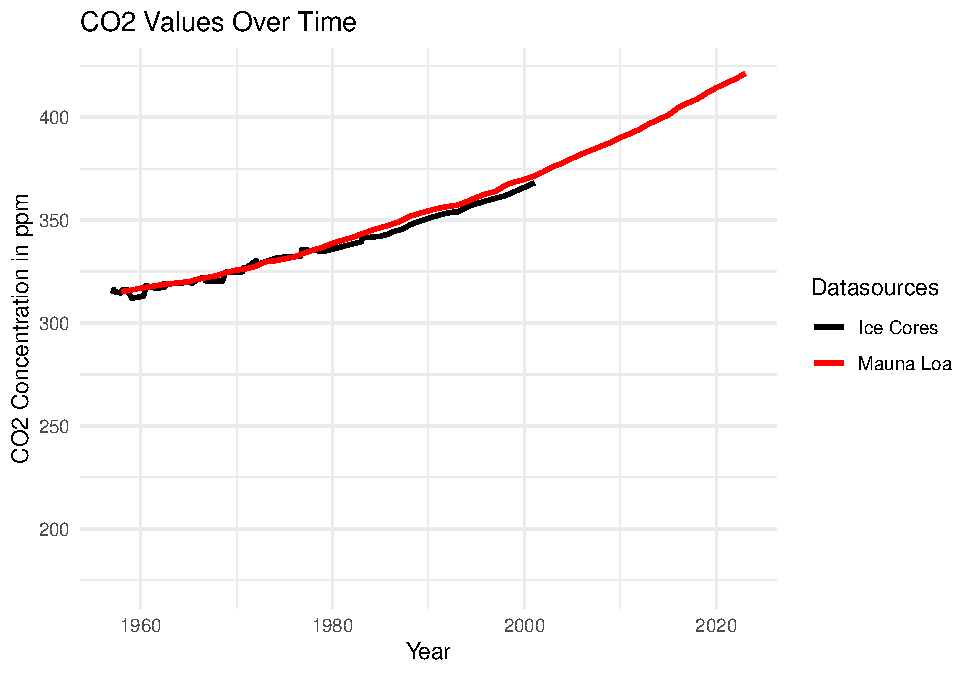
\includegraphics{data_wrangling_files/figure-latex/unnamed-chunk-13-1.pdf}

\hypertarget{data-correction-and-new-timeline}{%
\subsection{Data-Correction and new
Timeline}\label{data-correction-and-new-timeline}}

by computing offset, interpolation\ldots{} todo: write description, what
I do and why

\begin{Shaded}
\begin{Highlighting}[]
\CommentTok{\# define overlapping period}

\NormalTok{overlap\_period }\OtherTok{\textless{}{-}} \FunctionTok{c}\NormalTok{(}\DecValTok{1958}\NormalTok{,}\DecValTok{2001}\NormalTok{) }\CommentTok{\# start and end of overlapping period}

\CommentTok{\#to do: extract row where dataframe has certain value, to later be able to generate a generic function}
\DocumentationTok{\#\#\#\#\#\#\#\#\#\#\#\#\#\#\#\#\#\#\#\#\#\#\#\#\#\#\#\#\#\#\#\#\#\#\#\#\#\#\#\#\#\#\#\#\#\#\#\#\#\#}
\DocumentationTok{\#\#\#\#\#\#\#\#\#\#\#\#\#\#\#\#\#\#\#\#\#\#\#\#\#\#\#\#\#\#\#\#\#\#\#\#\#\#\#\#\#\#\#\#\#\#\#\#\#\#\#\#}

\NormalTok{i\_overlap\_period }\OtherTok{\textless{}{-}} \FunctionTok{filter}\NormalTok{(co2\_ice\_cores, year }\SpecialCharTok{\textgreater{}=}\NormalTok{ overlap\_period[}\DecValTok{1}\NormalTok{] }\SpecialCharTok{\&}\NormalTok{ year }\SpecialCharTok{\textless{}=}\NormalTok{ overlap\_period[}\DecValTok{2}\NormalTok{]) }
\NormalTok{m\_overlap\_period }\OtherTok{\textless{}{-}} \FunctionTok{filter}\NormalTok{(co2\_mauna\_loa, year }\SpecialCharTok{\textgreater{}=}\NormalTok{ overlap\_period[}\DecValTok{1}\NormalTok{] }\SpecialCharTok{\&}\NormalTok{ year }\SpecialCharTok{\textless{}=}\NormalTok{ overlap\_period[}\DecValTok{2}\NormalTok{])}

\CommentTok{\# calculate the means of the two datasets over this period}

\NormalTok{i\_co2\_mean }\OtherTok{\textless{}{-}} \FunctionTok{mean}\NormalTok{(i\_overlap\_period}\SpecialCharTok{$}\NormalTok{co2) }\CommentTok{\# mean over overlapping period ice{-}cores}
\NormalTok{m\_co2\_mean }\OtherTok{\textless{}{-}} \FunctionTok{mean}\NormalTok{(m\_overlap\_period}\SpecialCharTok{$}\NormalTok{co2) }\CommentTok{\# mean over overlapping period mauna{-}loa}

\CommentTok{\# mean difference}

\NormalTok{offset }\OtherTok{\textless{}{-}}\NormalTok{ m\_co2\_mean }\SpecialCharTok{{-}}\NormalTok{ i\_co2\_mean}

\CommentTok{\# add offset to ice{-}core dataset}

\ControlFlowTok{for}\NormalTok{ ( i }\ControlFlowTok{in} \DecValTok{1}\SpecialCharTok{:}\DecValTok{50}\NormalTok{)\{}
  
\NormalTok{  co2\_ice\_cores[i,}\DecValTok{2}\NormalTok{] }\OtherTok{\textless{}{-}} \FunctionTok{as.numeric}\NormalTok{(co2\_ice\_cores[i,}\DecValTok{2}\NormalTok{]) }\SpecialCharTok{+}\NormalTok{ offset}
  
\NormalTok{\} }

\CommentTok{\# plot of the corrected timeline consisting of the two datasets}

\FunctionTok{ggplot}\NormalTok{() }\SpecialCharTok{+}
  \FunctionTok{geom\_line}\NormalTok{(}\AttributeTok{data=}\NormalTok{ co2\_ice\_cores, }\FunctionTok{aes}\NormalTok{(}\AttributeTok{x =}\NormalTok{ year, }\AttributeTok{y =}\NormalTok{ co2, }\AttributeTok{color =} \StringTok{"Ice Cores"}\NormalTok{), }\AttributeTok{size =} \DecValTok{1}\NormalTok{) }\SpecialCharTok{+}
  \FunctionTok{geom\_line}\NormalTok{(}\AttributeTok{data =}\NormalTok{ co2\_mauna\_loa, }\FunctionTok{aes}\NormalTok{(}\AttributeTok{x =}\NormalTok{ year, }\AttributeTok{y =}\NormalTok{ co2, }\AttributeTok{color =} \StringTok{"Mauna Loa"}\NormalTok{), }\AttributeTok{size =} \DecValTok{1}\NormalTok{) }\SpecialCharTok{+}
  \FunctionTok{labs}\NormalTok{(}\AttributeTok{title =} \StringTok{"CO2 Values Over Time"}\NormalTok{,}
       \AttributeTok{x =} \StringTok{"Year"}\NormalTok{,}
       \AttributeTok{y =} \StringTok{"CO2 Concentration in ppm"}\NormalTok{) }\SpecialCharTok{+}
  \FunctionTok{scale\_color\_manual}\NormalTok{(}\AttributeTok{values =} \FunctionTok{c}\NormalTok{(}\StringTok{"Ice Cores"} \OtherTok{=} \StringTok{"black"}\NormalTok{, }\StringTok{"Mauna Loa"} \OtherTok{=} \StringTok{"red"}\NormalTok{),}
                     \AttributeTok{name =} \StringTok{"Datasources"}\NormalTok{) }\SpecialCharTok{+}
  \FunctionTok{xlim}\NormalTok{(}\DecValTok{1958}\NormalTok{, }\DecValTok{2023}\NormalTok{) }\SpecialCharTok{+}
  \FunctionTok{theme\_minimal}\NormalTok{()}
\end{Highlighting}
\end{Shaded}

\begin{verbatim}
## Warning: Removed 1851 rows containing missing values (`geom_line()`).
\end{verbatim}

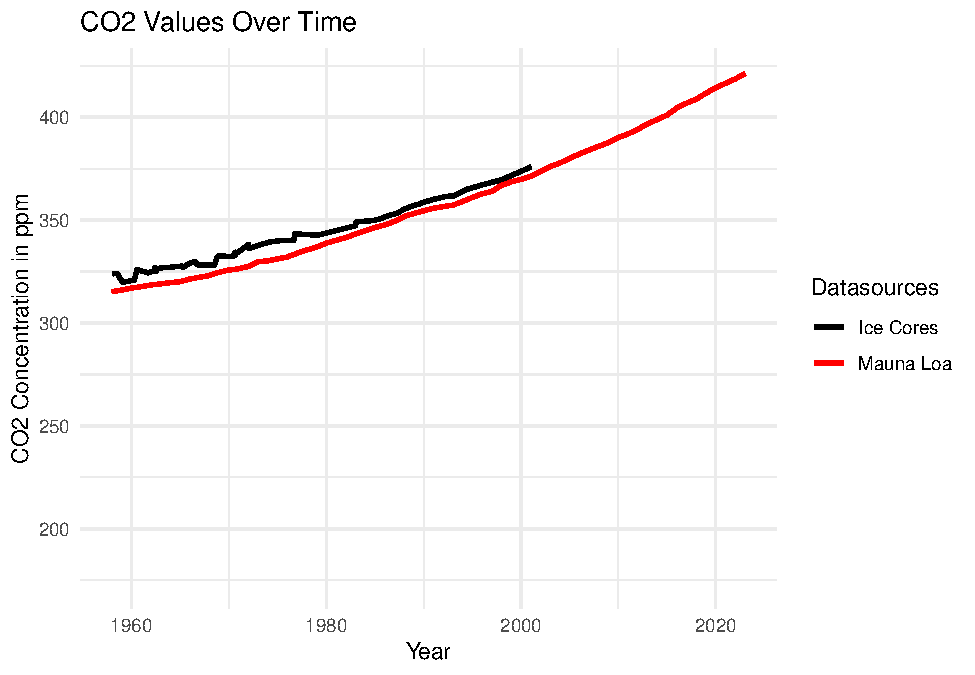
\includegraphics{data_wrangling_files/figure-latex/unnamed-chunk-14-1.pdf}

\begin{Shaded}
\begin{Highlighting}[]
\CommentTok{\# putting the two CO2{-}datasets together }

\NormalTok{co2\_timeline }\OtherTok{\textless{}{-}} \FunctionTok{merge}\NormalTok{(co2\_mauna\_loa, co2\_ice\_cores, }\AttributeTok{by =} \StringTok{"year"}\NormalTok{, }\AttributeTok{all =} \ConstantTok{TRUE}\NormalTok{)}

\CommentTok{\# rename the columns}

\FunctionTok{colnames}\NormalTok{(co2\_timeline) }\OtherTok{\textless{}{-}} \FunctionTok{c}\NormalTok{(}\StringTok{"year"}\NormalTok{, }\StringTok{"co2\_mauna\_loa"}\NormalTok{, }\StringTok{"co2\_ice\_cores"}\NormalTok{)}

\CommentTok{\# aggregate to one column with co2{-}values if one column has a NA then take the value of the other column}
\CommentTok{\# if both columns have values take the linear interpolation of the two points}

\NormalTok{one\_var\_co2\_timeline }\OtherTok{\textless{}{-}}\NormalTok{ co2\_timeline }\SpecialCharTok{|\textgreater{}}
  \FunctionTok{mutate}\NormalTok{(}\AttributeTok{aggregated\_column =} \FunctionTok{coalesce}\NormalTok{(co2\_mauna\_loa, co2\_ice\_cores))}


\CommentTok{\# non{-}continuous plot}

\FunctionTok{ggplot}\NormalTok{(}\AttributeTok{data =}\NormalTok{ co2\_timeline) }\SpecialCharTok{+}
  \FunctionTok{geom\_line}\NormalTok{(}\FunctionTok{aes}\NormalTok{(}\AttributeTok{x =}\NormalTok{ year, }\AttributeTok{y =}\NormalTok{ co2\_ice\_cores, }\AttributeTok{color =} \StringTok{"Ice{-}cores"}\NormalTok{), }\AttributeTok{size =} \DecValTok{1}\NormalTok{) }\SpecialCharTok{+}
  \FunctionTok{geom\_line}\NormalTok{(}\FunctionTok{aes}\NormalTok{(}\AttributeTok{x =}\NormalTok{ year, }\AttributeTok{y =}\NormalTok{ co2\_mauna\_loa, }\AttributeTok{color =} \StringTok{"Mauna{-}loa"}\NormalTok{), }\AttributeTok{size =} \DecValTok{1}\NormalTok{) }\SpecialCharTok{+}
  \FunctionTok{labs}\NormalTok{(}\AttributeTok{title =} \StringTok{"CO2 Values Over Time"}\NormalTok{,}
       \AttributeTok{x =} \StringTok{"Year"}\NormalTok{,}
       \AttributeTok{y =} \StringTok{"CO2 Concentration in ppm"}\NormalTok{) }\SpecialCharTok{+}
  \FunctionTok{scale\_color\_manual}\NormalTok{(}\AttributeTok{name =} \StringTok{"Datasources"}\NormalTok{, }\AttributeTok{values =} \FunctionTok{c}\NormalTok{(}\StringTok{"Ice{-}cores"} \OtherTok{=} \StringTok{"black"}\NormalTok{, }\StringTok{"Mauna{-}loa"} \OtherTok{=} \StringTok{"red"}\NormalTok{)) }\SpecialCharTok{+}
  \FunctionTok{xlim}\NormalTok{(}\DecValTok{1950}\NormalTok{, }\DecValTok{2023}\NormalTok{) }\SpecialCharTok{+}
  \FunctionTok{theme\_minimal}\NormalTok{()}
\end{Highlighting}
\end{Shaded}

\begin{verbatim}
## Warning: Removed 1862 rows containing missing values (`geom_line()`).
\end{verbatim}

\begin{verbatim}
## Warning: Removed 1851 rows containing missing values (`geom_line()`).
\end{verbatim}

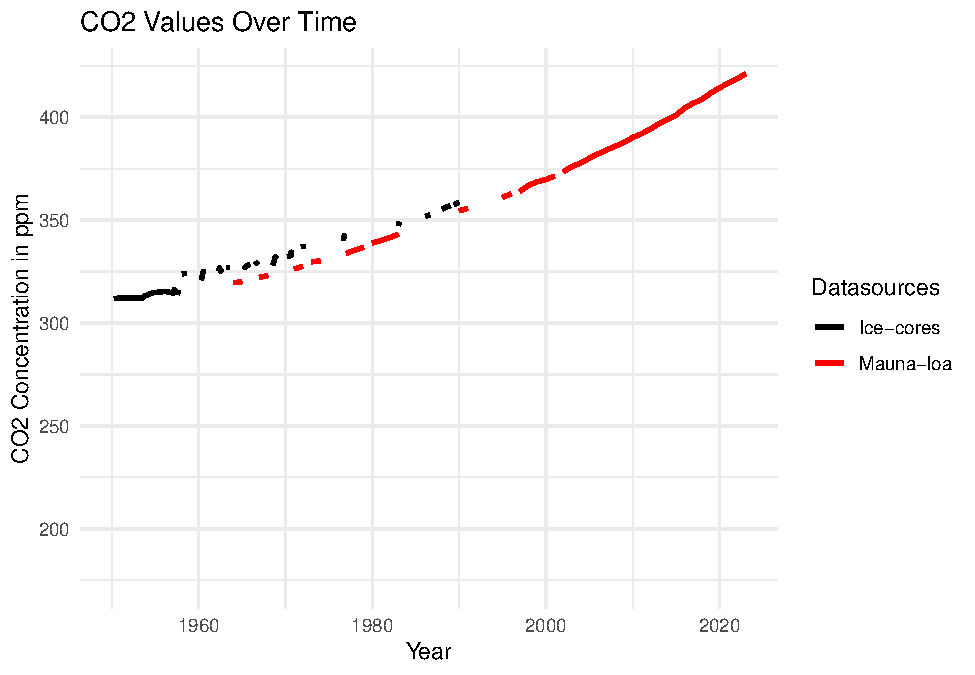
\includegraphics{data_wrangling_files/figure-latex/unnamed-chunk-15-1.pdf}

\begin{Shaded}
\begin{Highlighting}[]
\CommentTok{\# plot}

\FunctionTok{ggplot}\NormalTok{(}\AttributeTok{data =}\NormalTok{ one\_var\_co2\_timeline) }\SpecialCharTok{+}
  \FunctionTok{geom\_line}\NormalTok{(}\FunctionTok{aes}\NormalTok{(}\AttributeTok{x =}\NormalTok{ year, }\AttributeTok{y =}\NormalTok{ aggregated\_column), }\AttributeTok{size =} \DecValTok{1}\NormalTok{) }\SpecialCharTok{+}
  \FunctionTok{labs}\NormalTok{(}\AttributeTok{title =} \StringTok{"CO2 Values Over Time"}\NormalTok{,}
       \AttributeTok{x =} \StringTok{"Year"}\NormalTok{,}
       \AttributeTok{y =} \StringTok{"CO2 Concentration in ppm"}\NormalTok{) }\SpecialCharTok{+}
  \FunctionTok{xlim}\NormalTok{(}\DecValTok{1950}\NormalTok{, }\DecValTok{2023}\NormalTok{) }\SpecialCharTok{+}
  \FunctionTok{theme\_minimal}\NormalTok{()}
\end{Highlighting}
\end{Shaded}

\begin{verbatim}
## Warning: Removed 1840 rows containing missing values (`geom_line()`).
\end{verbatim}

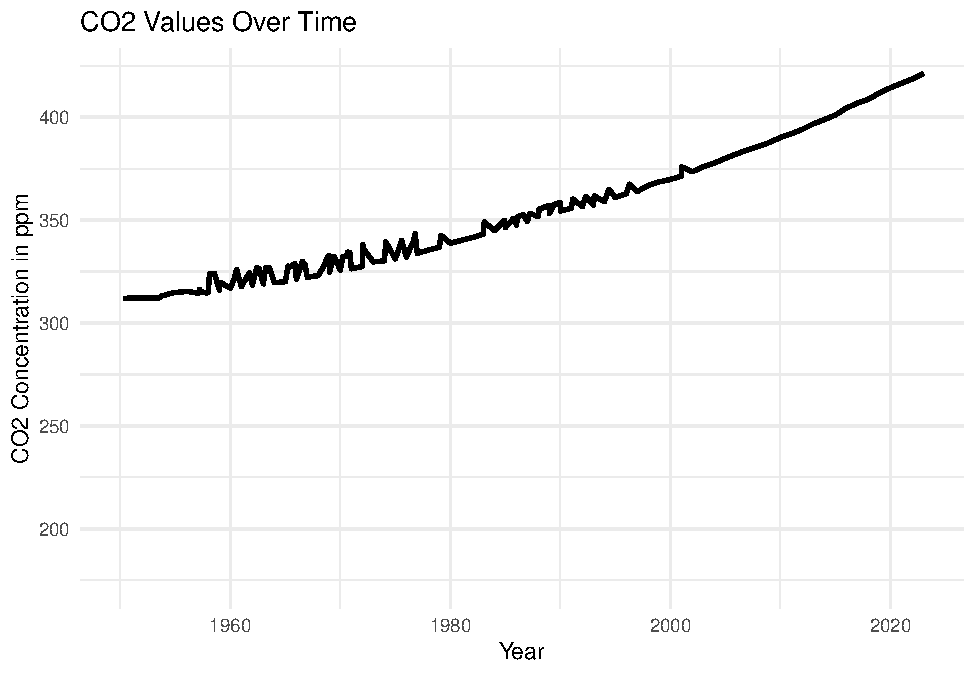
\includegraphics{data_wrangling_files/figure-latex/unnamed-chunk-15-2.pdf}

\emph{Frage}: Was mache ich nachdem ich den Offset gemacht habe? Ist ja
nicht wirklich eine schöne Kurve. Mein Ziel ist eine oder mehrere schöne
Visualisierungen und dann eine Analyse machen mit der Rate-of-Change (?)

\hypertarget{fancy-visualisations}{%
\subsubsection{Fancy Visualisations}\label{fancy-visualisations}}

(funktioniert noch nicht, will eine animierte Visualisierung machen
evt.)

\begin{Shaded}
\begin{Highlighting}[]
\CommentTok{\# libraries:}
\FunctionTok{library}\NormalTok{(ggplot2)}
\FunctionTok{library}\NormalTok{(gganimate)}
\end{Highlighting}
\end{Shaded}

\begin{verbatim}
## No renderer backend detected. gganimate will default to writing frames to separate files
## Consider installing:
## - the `gifski` package for gif output
## - the `av` package for video output
## and restarting the R session
\end{verbatim}

\begin{Shaded}
\begin{Highlighting}[]
\FunctionTok{library}\NormalTok{(transformr)}
\CommentTok{\#library(hrbrthemes)}

\NormalTok{transition\_states }\OtherTok{\textless{}{-}} \FunctionTok{seq}\NormalTok{(}\DecValTok{1950}\NormalTok{, }\DecValTok{2023}\NormalTok{, }\AttributeTok{by =} \DecValTok{5}\NormalTok{)}

\NormalTok{plot }\OtherTok{\textless{}{-}} \FunctionTok{ggplot}\NormalTok{(}\AttributeTok{data =}\NormalTok{ co2\_timeline) }\SpecialCharTok{+}
  \FunctionTok{geom\_line}\NormalTok{(}\FunctionTok{aes}\NormalTok{(}\AttributeTok{x =}\NormalTok{ year, }\AttributeTok{y =}\NormalTok{ co2\_ice\_cores, }\AttributeTok{color =} \StringTok{"Ice Cores"}\NormalTok{), }\AttributeTok{size =} \DecValTok{1}\NormalTok{) }\SpecialCharTok{+}
  \FunctionTok{geom\_line}\NormalTok{(}\FunctionTok{aes}\NormalTok{(}\AttributeTok{x =}\NormalTok{ year, }\AttributeTok{y =}\NormalTok{ co2\_mauna\_loa, }\AttributeTok{color =} \StringTok{"Mauna Loa"}\NormalTok{), }\AttributeTok{size =} \DecValTok{1}\NormalTok{) }\SpecialCharTok{+}
  \FunctionTok{labs}\NormalTok{(}\AttributeTok{title =} \StringTok{"CO2 Values Over Time"}\NormalTok{,}
       \AttributeTok{x =} \StringTok{"Year"}\NormalTok{,}
       \AttributeTok{y =} \StringTok{"CO2 Concentration in ppm"}\NormalTok{) }\SpecialCharTok{+}
  \FunctionTok{scale\_color\_manual}\NormalTok{(}\AttributeTok{values =} \FunctionTok{c}\NormalTok{(}\StringTok{"Ice Cores"} \OtherTok{=} \StringTok{"black"}\NormalTok{, }\StringTok{"Mauna Loa"} \OtherTok{=} \StringTok{"red"}\NormalTok{),}
                     \AttributeTok{name =} \StringTok{"Datasources"}\NormalTok{) }\SpecialCharTok{+}
  \FunctionTok{xlim}\NormalTok{(}\DecValTok{1958}\NormalTok{, }\DecValTok{2023}\NormalTok{) }\SpecialCharTok{+}
  \FunctionTok{theme\_minimal}\NormalTok{()}\CommentTok{\#+}
  \CommentTok{\#transition\_reveal(year)+}
  \CommentTok{\#transition\_states(transition\_states, transition\_length = 1, state\_length = 1, wrap = FALSE)}


\CommentTok{\# Save at gif:}
\CommentTok{\#anim\_save("co2{-}animation.gif", animation = plot)}
\end{Highlighting}
\end{Shaded}

\hypertarget{analysis}{%
\subsection{Analysis}\label{analysis}}

\begin{itemize}
\tightlist
\item
  überlappende Periode der Datensätze herausfinden
\item
  means der beiden Datensätze ausrechnen
\item
  der zuverlässigere Datensatz auswählen und die Abweichung der beiden
  means beim verbleibenden Datensatz dazurechnen
\item
  änderungsraten analyse mit linear fit
\end{itemize}

(ab hier nicht mehr lesen, wäre das Gleiche mit der Temperatur)

\hypertarget{temperature-timeline}{%
\subsection{Temperature timeline}\label{temperature-timeline}}

\begin{Shaded}
\begin{Highlighting}[]
\CommentTok{\# putting the four temperature{-}datasets together }

\NormalTok{temp\_timeline }\OtherTok{\textless{}{-}} \FunctionTok{merge}\NormalTok{(temp\_NOAA\_recentEra, temp\_pages2k, }\AttributeTok{by =} \StringTok{"year"}\NormalTok{, }\AttributeTok{all =} \ConstantTok{TRUE}\NormalTok{)}
\NormalTok{temp\_timeline }\OtherTok{\textless{}{-}} \FunctionTok{merge}\NormalTok{(temp\_timeline, temp\_antarctica, }\AttributeTok{by =} \StringTok{"year"}\NormalTok{, }\AttributeTok{all =} \ConstantTok{TRUE}\NormalTok{ )}
\NormalTok{temp\_timeline }\OtherTok{\textless{}{-}} \FunctionTok{merge}\NormalTok{(temp\_timeline, temp\_800KYr, }\AttributeTok{by =} \StringTok{"year"}\NormalTok{, }\AttributeTok{all =} \ConstantTok{TRUE}\NormalTok{ )}
\end{Highlighting}
\end{Shaded}

\begin{verbatim}
## Warning in merge.data.frame(temp_timeline, temp_800KYr, by = "year", all =
## TRUE): column names 'temp.x', 'temp.y' are duplicated in the result
\end{verbatim}

\begin{Shaded}
\begin{Highlighting}[]
\CommentTok{\# rename the columns}

\FunctionTok{colnames}\NormalTok{(temp\_timeline) }\OtherTok{\textless{}{-}} \FunctionTok{c}\NormalTok{(}\StringTok{"year"}\NormalTok{, }\StringTok{"temp\_NOAA\_recentEra"}\NormalTok{, }\StringTok{"temp\_pages2k"}\NormalTok{, }\StringTok{"temp\_antarctica"}\NormalTok{, }\StringTok{"temp\_800KYr"}\NormalTok{)}

\CommentTok{\# plot whole temperature timeline}

\FunctionTok{ggplot}\NormalTok{(}\AttributeTok{data =}\NormalTok{ temp\_timeline) }\SpecialCharTok{+}
  \FunctionTok{geom\_line}\NormalTok{(}\FunctionTok{aes}\NormalTok{(}\AttributeTok{x =}\NormalTok{ year, }\AttributeTok{y =}\NormalTok{ temp\_NOAA\_recentEra, }\AttributeTok{color =} \StringTok{"Temp\_NOAA\_recentEra"}\NormalTok{), }\AttributeTok{size =} \DecValTok{1}\NormalTok{) }\SpecialCharTok{+}
  \FunctionTok{geom\_line}\NormalTok{(}\FunctionTok{aes}\NormalTok{(}\AttributeTok{x =}\NormalTok{ year, }\AttributeTok{y =}\NormalTok{ temp\_pages2k, }\AttributeTok{color =} \StringTok{"Temp\_pages2k"}\NormalTok{), }\AttributeTok{size =} \DecValTok{1}\NormalTok{) }\SpecialCharTok{+}
  \FunctionTok{geom\_line}\NormalTok{(}\FunctionTok{aes}\NormalTok{(}\AttributeTok{x =}\NormalTok{ year, }\AttributeTok{y =}\NormalTok{ temp\_800KYr, }\AttributeTok{color =} \StringTok{"Temp\_800KYr"}\NormalTok{), }\AttributeTok{size =} \DecValTok{1}\NormalTok{) }\SpecialCharTok{+}
  \FunctionTok{labs}\NormalTok{(}\AttributeTok{title =} \StringTok{"Temperature Values Over Time"}\NormalTok{,}
       \AttributeTok{x =} \StringTok{"Year"}\NormalTok{,}
       \AttributeTok{y =} \StringTok{"Temperature in °C"}\NormalTok{) }\SpecialCharTok{+}
  \FunctionTok{scale\_color\_manual}\NormalTok{(}\AttributeTok{name =} \StringTok{"Datasources"}\NormalTok{, }\AttributeTok{values =} \FunctionTok{c}\NormalTok{(}\StringTok{"Temp\_NOAA\_recentEra"} \OtherTok{=} \StringTok{"lightblue"}\NormalTok{, }\StringTok{"Temp\_pages2k"} \OtherTok{=} \StringTok{"pink"}\NormalTok{, }\StringTok{"Temp\_800KYr"} \OtherTok{=} \StringTok{"lightgreen"}\NormalTok{ )) }\SpecialCharTok{+}
  \FunctionTok{theme\_minimal}\NormalTok{()}
\end{Highlighting}
\end{Shaded}

\begin{verbatim}
## Warning: Removed 8581 rows containing missing values (`geom_line()`).
\end{verbatim}

\begin{verbatim}
## Warning: Removed 6620 rows containing missing values (`geom_line()`).
\end{verbatim}

\begin{verbatim}
## Warning: Removed 111 rows containing missing values (`geom_line()`).
\end{verbatim}

\includegraphics{data_wrangling_files/figure-latex/unnamed-chunk-17-1.pdf}

\begin{Shaded}
\begin{Highlighting}[]
\CommentTok{\# create subset of the dataframe for better visualizations of the overlapping sections}

\NormalTok{overlap\_temp\_timeline }\OtherTok{\textless{}{-}}\NormalTok{ temp\_timeline[temp\_timeline}\SpecialCharTok{$}\NormalTok{year }\SpecialCharTok{\textgreater{}=} \DecValTok{1850} \SpecialCharTok{\&}\NormalTok{ co2\_timeline}\SpecialCharTok{$}\NormalTok{year }\SpecialCharTok{\textless{}=} \DecValTok{2002}\NormalTok{, ]}
\end{Highlighting}
\end{Shaded}

\begin{verbatim}
## Warning in temp_timeline$year >= 1850 & co2_timeline$year <= 2002: Länge des längeren Objektes
##       ist kein Vielfaches der Länge des kürzeren Objektes
\end{verbatim}

\begin{Shaded}
\begin{Highlighting}[]
\CommentTok{\# plot}

\FunctionTok{ggplot}\NormalTok{(}\AttributeTok{data =}\NormalTok{ overlap\_temp\_timeline) }\SpecialCharTok{+}
  \FunctionTok{geom\_line}\NormalTok{(}\FunctionTok{aes}\NormalTok{(}\AttributeTok{x =}\NormalTok{ year, }\AttributeTok{y =}\NormalTok{ temp\_NOAA\_recentEra, }\AttributeTok{color =} \StringTok{"Temp\_NOAA\_recentEra"}\NormalTok{), }\AttributeTok{size =} \DecValTok{1}\NormalTok{) }\SpecialCharTok{+}
  \FunctionTok{geom\_line}\NormalTok{(}\FunctionTok{aes}\NormalTok{(}\AttributeTok{x =}\NormalTok{ year, }\AttributeTok{y =}\NormalTok{ temp\_pages2k, }\AttributeTok{color =} \StringTok{"Temp\_pages2K"}\NormalTok{), }\AttributeTok{size =} \DecValTok{1}\NormalTok{) }\SpecialCharTok{+}
  \FunctionTok{geom\_line}\NormalTok{(}\FunctionTok{aes}\NormalTok{(}\AttributeTok{x =}\NormalTok{ year, }\AttributeTok{y =}\NormalTok{ temp\_800KYr, }\AttributeTok{color =} \StringTok{"Temp\_800KYr"}\NormalTok{), }\AttributeTok{size =} \DecValTok{1}\NormalTok{) }\SpecialCharTok{+}
  \FunctionTok{labs}\NormalTok{(}\AttributeTok{title =} \StringTok{"CO2 Values Over Time"}\NormalTok{,}
       \AttributeTok{x =} \StringTok{"Year"}\NormalTok{,}
       \AttributeTok{y =} \StringTok{"CO2 Concentration in ppm"}\NormalTok{) }\SpecialCharTok{+}
  \FunctionTok{scale\_color\_manual}\NormalTok{(}\AttributeTok{name =} \StringTok{"Datasources"}\NormalTok{, }\AttributeTok{values =} \FunctionTok{c}\NormalTok{(}\StringTok{"Temp\_NOAA\_recentEra"} \OtherTok{=} \StringTok{"lightblue"}\NormalTok{, }\StringTok{"Temp\_pages2K"} \OtherTok{=} \StringTok{"pink"}\NormalTok{, }\StringTok{"Temp\_800KYr"} \OtherTok{=} \StringTok{"lightgreen"}\NormalTok{)) }\SpecialCharTok{+}
  \FunctionTok{theme\_minimal}\NormalTok{()}
\end{Highlighting}
\end{Shaded}

\begin{verbatim}
## Warning: Removed 22 rows containing missing values (`geom_line()`).
\end{verbatim}

\begin{verbatim}
## Warning: Removed 112 rows containing missing values (`geom_line()`).
\end{verbatim}

\includegraphics{data_wrangling_files/figure-latex/unnamed-chunk-18-1.pdf}

\hypertarget{citations}{%
\section{Citations}\label{citations}}

Average temperature of 1901-2000
\url{https://www.ncei.noaa.gov/access/monitoring/monthly-report/global/202013\#}:\textasciitilde:text=The\%201901\%E2\%80\%932000\%20average\%20combined,C\%20(60.9\%C2\%B0F).

The average temperature over the period 1960-1990 was 14°C
\url{https://www.un.org/sustainabledevelopment/blog/2016/01/wmo-confirms-2015-as-hottest-year-on-record/\#}:\textasciitilde:text=WMO\%20uses\%201961\%2D1990\%20as,period\%20was\%2014\%C2\%B0C.

\end{document}
